\documentclass[fleqn, 10pt]{article}

% Paquetes necesarios
\usepackage[utf8]{inputenc}
\usepackage[spanish]{babel}
\usepackage{amsthm}
\usepackage{nccmath} %Para centrar ecuaciones
\usepackage{enumitem}
\usepackage{graphicx}
\usepackage{verbatim}
\usepackage{algpseudocode}



\DeclareMathAlphabet{\pazocal}{OMS}{zplm}{m}{n}
\newcommand{\Lb}{\pazocal{L}}


\theoremstyle{plain}
\newtheorem{proposicion}{Proposición}

\theoremstyle{definition}
\newtheorem{definition}{Definición}[section]
\newtheorem{example}{Ejemplo}[section]

%Definimos el título
\title{Teoría de Autómatas y Lenguajes Formales\\[.4\baselineskip]Práctica 2: Autómatas en JFLAP}
\author{Alba Robles Morales}
\date{27/10/2022}



%Comienzo del documento
\begin{document}

%Generamos el título
\maketitle

\section{Define una Turing Machine que sea solución del ejercicio 3.4 de la relación de problemas. }

\begin{center}
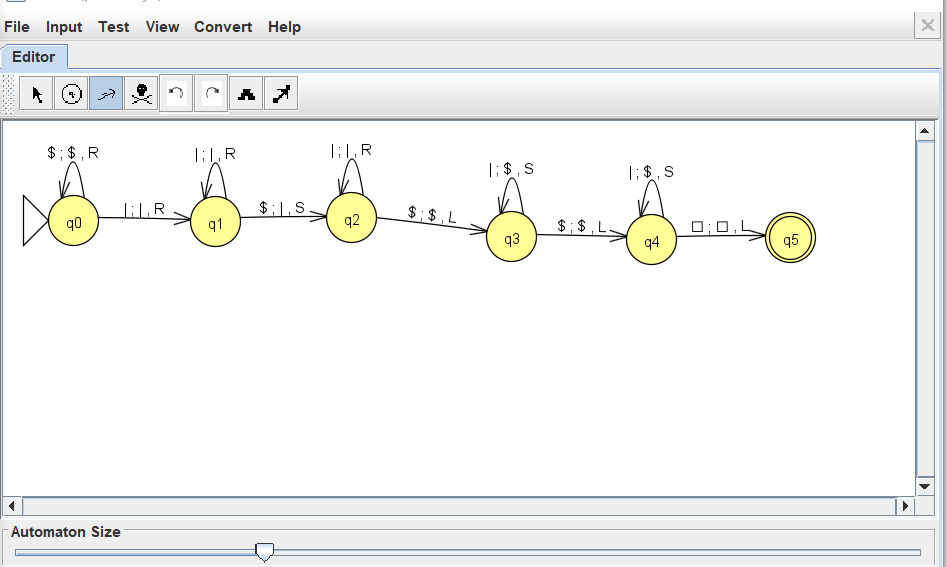
\includegraphics[width=11cm, height=8cm]{1_pract3.png}
\end{center}

\section {Define una función recursiva para la suma de tres valores.}

Para que una función recursiva sume tres números lo que haremos será una función que primero sume dos valores y el resultado de este lo sume con el tercero.

\begin{equation}
suma=<<\pi^1_1|\sigma(\pi^3_3)>|\sigma(\pi^4_4)>
\end {equation}
\begin{center}
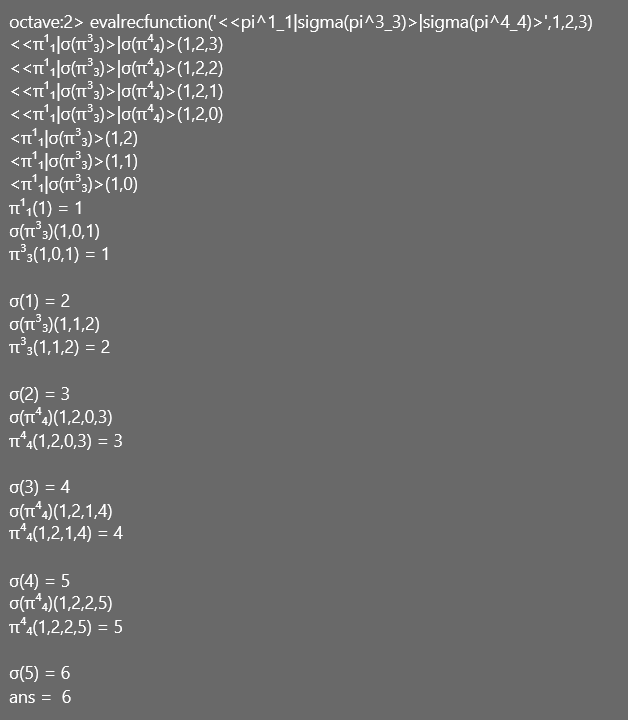
\includegraphics[width=12cm, height=10cm]{talf_pract3_ej2.png}
\end{center}


\section {Implementa un programa while que compute la suma de tres valores.}

\begin{algorithmic}
\While{X2!=0 }
\While{X3!=0 }

	\\x1:=x1+1;
	\\x3:=x3-1;
\EndWhile
\\x1:=x1+1;
\\x2:=x2-1;
\EndWhile
\end{algorithmic}

\end{document}